\documentclass[12pt,a4paper]{report}

% ═══════════════════════════════════════════
% PACKAGES
% ═══════════════════════════════════════════
\usepackage[utf8]{inputenc}
\usepackage[T1]{fontenc}
\usepackage[french]{babel}
\usepackage{lmodern}
\usepackage{amsmath, amsfonts, amssymb}
\usepackage{graphicx}
\usepackage{geometry}
\usepackage{hyperref}
\usepackage{booktabs}
\usepackage{caption}
\usepackage{subcaption}
\usepackage{float}
\usepackage{xcolor}
\usepackage{fancyhdr}
\usepackage{enumitem}
\usepackage{tabularx}
\usepackage{multirow}
\usepackage{listings}
\usepackage{setspace}
\usepackage{parskip}

% ═══════════════════════════════════════════
% CONFIGURATION
% ═══════════════════════════════════════════
\geometry{top=2.5cm, bottom=2.5cm, left=3cm, right=2.5cm}
\setstretch{1.25}

\hypersetup{
    colorlinks=true,
    linkcolor=blue!70!black,
    citecolor=green!50!black,
    urlcolor=cyan!70!black,
    pdftitle={Rapport PFM — IDS par Machine Learning},
}

\pagestyle{fancy}
\fancyhf{}
\fancyhead[L]{\small\nouppercase{\leftmark}}
\fancyhead[R]{\small Projet de Fin de Module}
\fancyfoot[C]{\thepage}
\renewcommand{\headrulewidth}{0.4pt}
\renewcommand{\footrulewidth}{0pt}

% Style des listings code
\lstset{
    basicstyle=\small\ttfamily,
    breaklines=true,
    frame=single,
    backgroundcolor=\color{gray!5},
    rulecolor=\color{gray!30},
    keywordstyle=\color{blue!70!black},
    commentstyle=\color{green!50!black},
    stringstyle=\color{red!60!black},
    numbers=left,
    numberstyle=\tiny\color{gray},
    numbersep=8pt,
    tabsize=4,
    showstringspaces=false,
}

\begin{document}

% ═══════════════════════════════════════════
% PAGE DE GARDE
% ═══════════════════════════════════════════
\begin{titlepage}
    \centering
    \vspace*{2cm}
    
    {\large\textsc{Master 1 — Module de Machine Learning}\par}
    \vspace{0.8cm}
    
    \rule{\textwidth}{0.5pt}
    \vspace{0.8cm}
    {\LARGE\bfseries Conception et Implémentation d'un\\Système de Détection d'Intrusions Réseau\\Basé sur le Machine Learning\par}
    \vspace{0.5cm}
    {\large\itshape Application MLOps sur le Dataset NSL-KDD\par}
    \vspace{0.3cm}
    \rule{\textwidth}{0.5pt}
    
    \vspace{2.5cm}
    
    {\large\textbf{Rapport de Projet de Fin de Module}\par}
    
    \vspace{3cm}
    
    {\large\textbf{Module :} Machine Learning\par}
    
    \vfill
    
    {\large Année universitaire 2025--2026\par}
\end{titlepage}

% ═══════════════════════════════════════════
% PAGES PRÉLIMINAIRES
% ═══════════════════════════════════════════
\pagenumbering{roman}

\chapter*{Résumé}
\addcontentsline{toc}{chapter}{Résumé}

La détection d'intrusions réseau constitue un enjeu majeur de la cybersécurité moderne. Les systèmes classiques, fondés sur des bases de signatures statiques, peinent à détecter les attaques inédites (\textit{Zero-Day}) et les comportements anormaux subtils. Ce projet propose une approche d'ingénierie appliquée, basée sur l'apprentissage automatique (\textit{Machine Learning}), pour la classification du trafic réseau en temps réel.

En utilisant le jeu de données de référence NSL-KDD, composé de 125\,973 connexions d'entraînement, nous avons développé un pipeline analytique complet. Le projet se concentre particulièrement sur les défis liés à la mise en production (MLOps) et à la gestion du déséquilibre extrême des classes. L'utilisation de la technique SMOTE (\textit{Synthetic Minority Over-sampling Technique}), intégrée de manière stricte dans la boucle de validation croisée pour éviter toute fuite de données, a permis de pallier la rareté critique de certaines attaques.

Les algorithmes ensemblistes Random Forest et XGBoost ont été retenus pour leur adéquation avec les données tabulaires hautement dimensionnelles. Les résultats montrent que XGBoost atteint une exactitude de 78,95\% et un F1-Score Macro de 0,631, avec des performances remarquables sur les classes minoritaires critiques : une précision de 97,11\% pour les attaques R2L et un F1-Score triplé (0,46) pour les attaques U2R. 

L'ensemble a été industrialisé sous forme d'une API REST asynchrone (FastAPI) minimisant la latence d'inférence, accompagnée d'un tableau de bord interactif, le tout conteneurisé via Docker pour un déploiement reproductible.

\textbf{Mots-clés :} Détection d'intrusions, Machine Learning Engineering, XGBoost, SMOTE, NSL-KDD, Déséquilibre de classes, MLOps, FastAPI, Docker.

\vspace{1cm}

\chapter*{Abstract}
\addcontentsline{toc}{chapter}{Abstract}

Network intrusion detection is a critical challenge in modern cybersecurity. Traditional signature-based systems fail to detect unknown (\textit{Zero-Day}) attacks and subtle anomalous behaviors. This project proposes an applied engineering approach, based on Machine Learning, for real-time network traffic classification.

Using the NSL-KDD benchmark dataset (125,973 training connections), we developed a complete analytical pipeline. The project specifically focuses on production deployment challenges (MLOps) and handling extreme class imbalance. The use of SMOTE (\textit{Synthetic Minority Over-sampling Technique}), strictly integrated within the cross-validation loop to prevent data leakage, addressed the critical scarcity of certain attacks.

Ensemble algorithms Random Forest and XGBoost were selected for their adequacy with highly dimensional tabular data. Results show that XGBoost achieves 78.95\% accuracy and a Macro F1-Score of 0.631, with remarkable performance on critical minority classes: 97.11\% precision for R2L attacks and a tripled F1-Score (0.46) for U2R attacks.

The system was industrialized as an asynchronous REST API (FastAPI) minimizing inference latency, accompanied by an interactive dashboard, all containerized via Docker for reproducible deployment.

\textbf{Keywords:} Intrusion Detection, Machine Learning Engineering, XGBoost, SMOTE, NSL-KDD, Class Imbalance, MLOps, FastAPI, Docker.

% ═══════════════════════════════════════════
% TABLE DES MATIÈRES
% ═══════════════════════════════════════════
\tableofcontents
\listoffigures
\listoftables

\newpage
\pagenumbering{arabic}

% ═══════════════════════════════════════════
% CHAPITRE 1 — INTRODUCTION
% ═══════════════════════════════════════════
\chapter{Introduction Générale}

\section{Contexte de la sécurité réseau}

L'ère numérique a transformé radicalement les infrastructures informatiques mondiales. Les réseaux d'entreprise sont devenus à la fois plus complexes et plus exposés aux menaces. Les cyberattaques modernes ne se limitent plus aux virus informatiques traditionnels, elles englobent un spectre sophistiqué : dénis de service (DoS), intrusions furtives (\textit{Remote-to-Local}), ou encore des élévations de privilèges (\textit{User-to-Root}) permettant à un attaquant d'obtenir un contrôle total.

Face à cette menace, les Systèmes de Détection d'Intrusions (IDS) classiques se basent sur des bibliothèques de signatures (comme Snort ou Suricata). Si cette approche est fiable contre les menaces documentées, elle reste aveugle face aux attaques \textit{Zero-Day}. Le \textit{Machine Learning} offre un paradigme comportemental puissant : identifier le trafic malveillant en apprenant les caractéristiques discriminantes directement à partir de grandes quantités de données historiques.

\section{Problématique d'ingénierie}

Ce projet ne se contente pas d'entraîner un modèle théorique, il vise à résoudre une problématique d'ingénierie globale :
\begin{quote}
    \textit{Comment concevoir, évaluer et déployer un pipeline ML robuste de détection d'intrusions capable de traiter en temps réel un trafic réseau déséquilibré, tout en évitant les biais méthodologiques inhérents aux environnements académiques ?}
\end{quote}

Cette problématique soulève plusieurs verrous technologiques :
\begin{enumerate}
    \item \textbf{Le déséquilibre extrême} : Comment détecter une attaque U2R qui représente moins de 0,04\% des données d'entraînement ?
    \item \textbf{L'intégrité de l'évaluation} : Comment appliquer des techniques de sur-échantillonnage (SMOTE) sans provoquer de fuite de données (\textit{Data Leakage}) ?
    \item \textbf{La latence d'inférence} : Comment industrialiser le modèle pour soutenir un débit de dizaines de milliers de paquets par seconde sans devenir un goulot d'étranglement réseau ?
\end{enumerate}

\section{Objectifs du projet}

Les objectifs de ce projet de fin de module s'inscrivent dans une démarche MLOps :
\begin{enumerate}[leftmargin=2cm]
    \item \textbf{Prétraitement rigoureux} : Analyse ciblée des variables du dataset NSL-KDD et encodage adapté pour les modèles tabulaires.
    \item \textbf{Gestion avancée du déséquilibre} : Implémentation de pipelines \texttt{imbalanced-learn} stricts.
    \item \textbf{Modélisation orientée performance} : Optimisation d'algorithmes ensemblistes de pointe (Random Forest, XGBoost) capables de gérer des données creuses sans surapprentissage.
    \item \textbf{Industrialisation} : Développement d'un microservice asynchrone (FastAPI) optimisé en mémoire, couplé à une interface de monitoring et conteneurisé.
\end{enumerate}


% ═══════════════════════════════════════════
% CHAPITRE 2 — DONNÉES ET DÉFIS MÉTIERS
% ═══════════════════════════════════════════
\chapter{Données et Défis Métiers}

\section{Le Dataset NSL-KDD : Une référence épurée}

Le projet s'appuie sur le dataset \textbf{NSL-KDD}, qui corrige les défauts majeurs (redondances massives) de son prédécesseur KDD Cup 1999. Il comprend 125\,973 connexions pour l'entraînement et 22\,544 pour le test.

Chaque connexion est décrite par 41 attributs. L'intérêt métier de ce dataset réside dans sa diversité : au-delà des en-têtes TCP/IP basiques, il intègre des caractéristiques \textbf{temporelles} et calculées sur des \textbf{fenêtres d'hôtes}. Ce sont précisément ces métriques (ex: le taux de connexions rejetées vers un même hôte sur une durée de 2 secondes) qui permettent aux algorithmes de déduire un comportement de scan ou de déni de service.

\section{Taxonomie et déséquilibre pathologique}

Les 39 types d'attaques originaux ont été agrégés en 5 classes macroscopiques. Le Tableau~\ref{tab:desequilibre} illustre le défi principal du projet : le déséquilibre pathologique.

\begin{table}[H]
    \centering
    \begin{tabular}{lccc}
        \toprule
        \textbf{Classe} & \textbf{Effectif (Train)} & \textbf{Proportion} & \textbf{Sévérité en production} \\
        \midrule
        Normal & 67\,343 & 53,46\% & N/A \\
        DoS & 45\,927 & 36,46\% & Élevée \\
        Probe & 11\,656 & 9,25\% & Modérée \\
        R2L & 995 & 0,79\% & Très Élevée \\
        U2R & 52 & 0,04\% & \textbf{Critique} \\
        \bottomrule
    \end{tabular}
    \caption{Distribution des classes et sévérité métier.}
    \label{tab:desequilibre}
\end{table}

La classe la plus dangereuse (U2R, élévation de privilèges conduisant à un contrôle total) est la moins représentée. Un modèle d'apprentissage classique l'ignorera purement et simplement pour minimiser sa perte globale.

\section{Le défi de généralisation du jeu de test}

Contrairement à la majorité des projets académiques où le jeu de test est un simple sous-ensemble de la distribution d'entraînement, le jeu de test du NSL-KDD contient des \textbf{attaques inédites} (ex: \texttt{mailbomb}, \texttt{mscan}, \texttt{apache2}). Cela force les modèles à \textit{généraliser} des motifs comportementaux au lieu de mémoriser des signatures.


% ═══════════════════════════════════════════
% CHAPITRE 3 — INGÉNIERIE ML ET ARCHITECTURE
% ═══════════════════════════════════════════
\chapter{Ingénierie ML et Justification des Choix}

Ce chapitre détaille les décisions architecturales et techniques prises pour construire un pipeline robuste, en s'éloignant des choix "par défaut".

\section{Prétraitement et dimensionnalité}

La préparation des données a nécessité deux transformations critiques :
\begin{enumerate}
    \item \textbf{Encodage One-Hot des variables textuelles} : Les attributs comme \texttt{service} ou \texttt{flag} ne possèdent pas de relation ordinale. Leur encodage a généré un espace d'entrée de 122 variables très creuses (sparse). Pour gérer l'asymétrie avec le jeu de test (qui contient des services non vus), la méthode \texttt{reindex()} de pandas a été employée pour garantir une stricte correspondance des dimensions.
    \item \textbf{Standardisation rigoureuse} : Un \texttt{StandardScaler} a été appliqué, ajusté \textit{uniquement} sur le jeu d'entraînement, puis sérialisé (\texttt{scaler.pkl}) pour l'inférence.
\end{enumerate}

\section{Prévention du Data Leakage avec SMOTE}

Pour traiter le déséquilibre extrême des attaques R2L et U2R, l'algorithme d'interpolation \textbf{SMOTE} a été retenu. Cependant, son implémentation est souvent source d'erreurs fatales en ML : appliquer SMOTE sur l'ensemble du dataset avant l'entraînement contamine la validation avec des données synthétiques.

\textbf{Choix architectural} : Nous avons intégré SMOTE à l'intérieur d'un objet \texttt{ImbPipeline} (issu de la librairie \texttt{imbalanced-learn}). Ainsi, lors de l'optimisation des hyperparamètres, la génération de données synthétiques s'effectue dynamiquement \textit{uniquement} sur les plis (folds) d'entraînement, préservant la pureté absolue du pli de validation.

Le compromis technique assumé ici est le \textbf{coût computationnel} : la génération dynamique de milliers de points à chaque itération allonge considérablement le temps d'entraînement.

\section{Justification du choix des algorithmes}

Plutôt que d'employer des algorithmes de Deep Learning (réseaux de neurones denses), très coûteux à mettre en production pour des données tabulaires, nous avons ciblé les modèles ensemblistes basés sur les arbres : \textbf{Random Forest} (Bagging) et \textbf{XGBoost} (Gradient Boosting).

Ces choix sont motivés par plusieurs facteurs d'ingénierie :
\begin{itemize}
    \item \textbf{Tolérance à la sparsité} : XGBoost possède des optimisations internes (Sparsity-aware Split Finding) excellentes pour gérer nos 122 variables encodées.
    \item \textbf{Latence d'inférence} : Les arbres de décision compilés permettent des temps de prédiction de l'ordre de la microseconde par connexion, un prérequis pour un IDS temps réel.
    \item \textbf{Résistance aux outliers} : Contrairement à la régression logistique, les arbres ne dépendent pas des distances euclidiennes et gèrent nativement les valeurs extrêmes communes dans le trafic réseau.
\end{itemize}

\section{Stratégie d'optimisation (RandomizedSearchCV)}

L'optimisation des hyperparamètres a été menée via une \texttt{RandomizedSearchCV} couplée à une validation croisée stratifiée (\texttt{StratifiedKFold}). La métrique cible choisie est le \textbf{F1-Score Macro}. Contrairement à l'exactitude globale (qui aurait favorisé la classe "Normal"), le F1-Score Macro force l'algorithme à accorder une importance égale à la classe U2R (52 exemples) et à la classe Normal (67\,343 exemples).


% ═══════════════════════════════════════════
% CHAPITRE 4 — RÉSULTATS
% ═══════════════════════════════════════════
\chapter{Résultats Expérimentaux et Analyse}

\section{Performances globales}

Le Tableau~\ref{tab:resultats-globaux} synthétise les scores sur le jeu de test NSL-KDD.

\begin{table}[H]
    \centering
    \begin{tabular}{lccc}
        \toprule
        \textbf{Métrique} & \textbf{Random Forest + SMOTE} & \textbf{XGBoost + SMOTE} & \textbf{Différence} \\
        \midrule
        Exactitude globale & 75,00\% & \textbf{78,95\%} & +3,95\% \\
        F1-Score Macro & 0,5342 & \textbf{0,6314} & +0,0972 \\
        F1-Score Pondéré & 0,7087 & \textbf{0,7582} & +0,0495 \\
        \bottomrule
    \end{tabular}
    \caption{Comparaison des scores globaux sur le jeu de test NSL-KDD.}
    \label{tab:resultats-globaux}
\end{table}

L'architecture XGBoost s'impose nettement, validant l'intérêt du \textit{Gradient Boosting} face au \textit{Bagging} pour corriger itérativement les erreurs sur les classes dures.

\section{Analyse granulaire des classes critiques}

La véritable valeur du pipeline réside dans sa capacité à identifier les attaques complexes. Le Tableau~\ref{tab:resultats-classe} détaille les performances.

\begin{table}[H]
    \centering
    \begin{tabular}{l|ccc|ccc}
        \toprule
        & \multicolumn{3}{c|}{\textbf{Random Forest + SMOTE}} & \multicolumn{3}{c}{\textbf{XGBoost + SMOTE}} \\
        \textbf{Classe} & Précision & Rappel & F1 & Précision & Rappel & F1 \\
        \midrule
        Normal & 0,6675 & 0,9667 & 0,7895 & 0,7236 & 0,9448 & 0,8196 \\
        DoS & 0,9543 & 0,6990 & 0,8071 & 0,9657 & 0,7704 & 0,8572 \\
        Probe & 0,7707 & 0,5753 & 0,6589 & 0,7449 & 0,7124 & 0,7283 \\
        R2L & 0,8333 & 0,2153 & 0,3423 & \textbf{0,9711} & 0,3153 & 0,4759 \\
        U2R & 0,1818 & 0,1463 & 0,1621 & \textbf{0,7188} & 0,3415 & \textbf{0,4630} \\
        \bottomrule
    \end{tabular}
    \caption{Performances détaillées par classe (Précision, Rappel, F1-Score).}
    \label{tab:resultats-classe}
\end{table}

\textbf{L'impact majeur de SMOTE + XGBoost} s'observe sur les attaques U2R : le F1-Score a quasiment triplé (0,16 vers 0,46), avec une précision étonnante de 71,88\%. Sur la classe R2L, XGBoost atteint une précision de 97,11\% (lorsque le modèle lève une alerte R2L, il a presque toujours raison). Le rappel (Recall) modeste de ces classes s'explique par les attaques inédites présentes dans le jeu de test.

\section{Matrices de confusion et analyse d'erreurs}

L'analyse de la matrice d'XGBoost (Figure~\ref{fig:confusion}) met en lumière la nature des erreurs.

\begin{figure}[H]
    \centering
    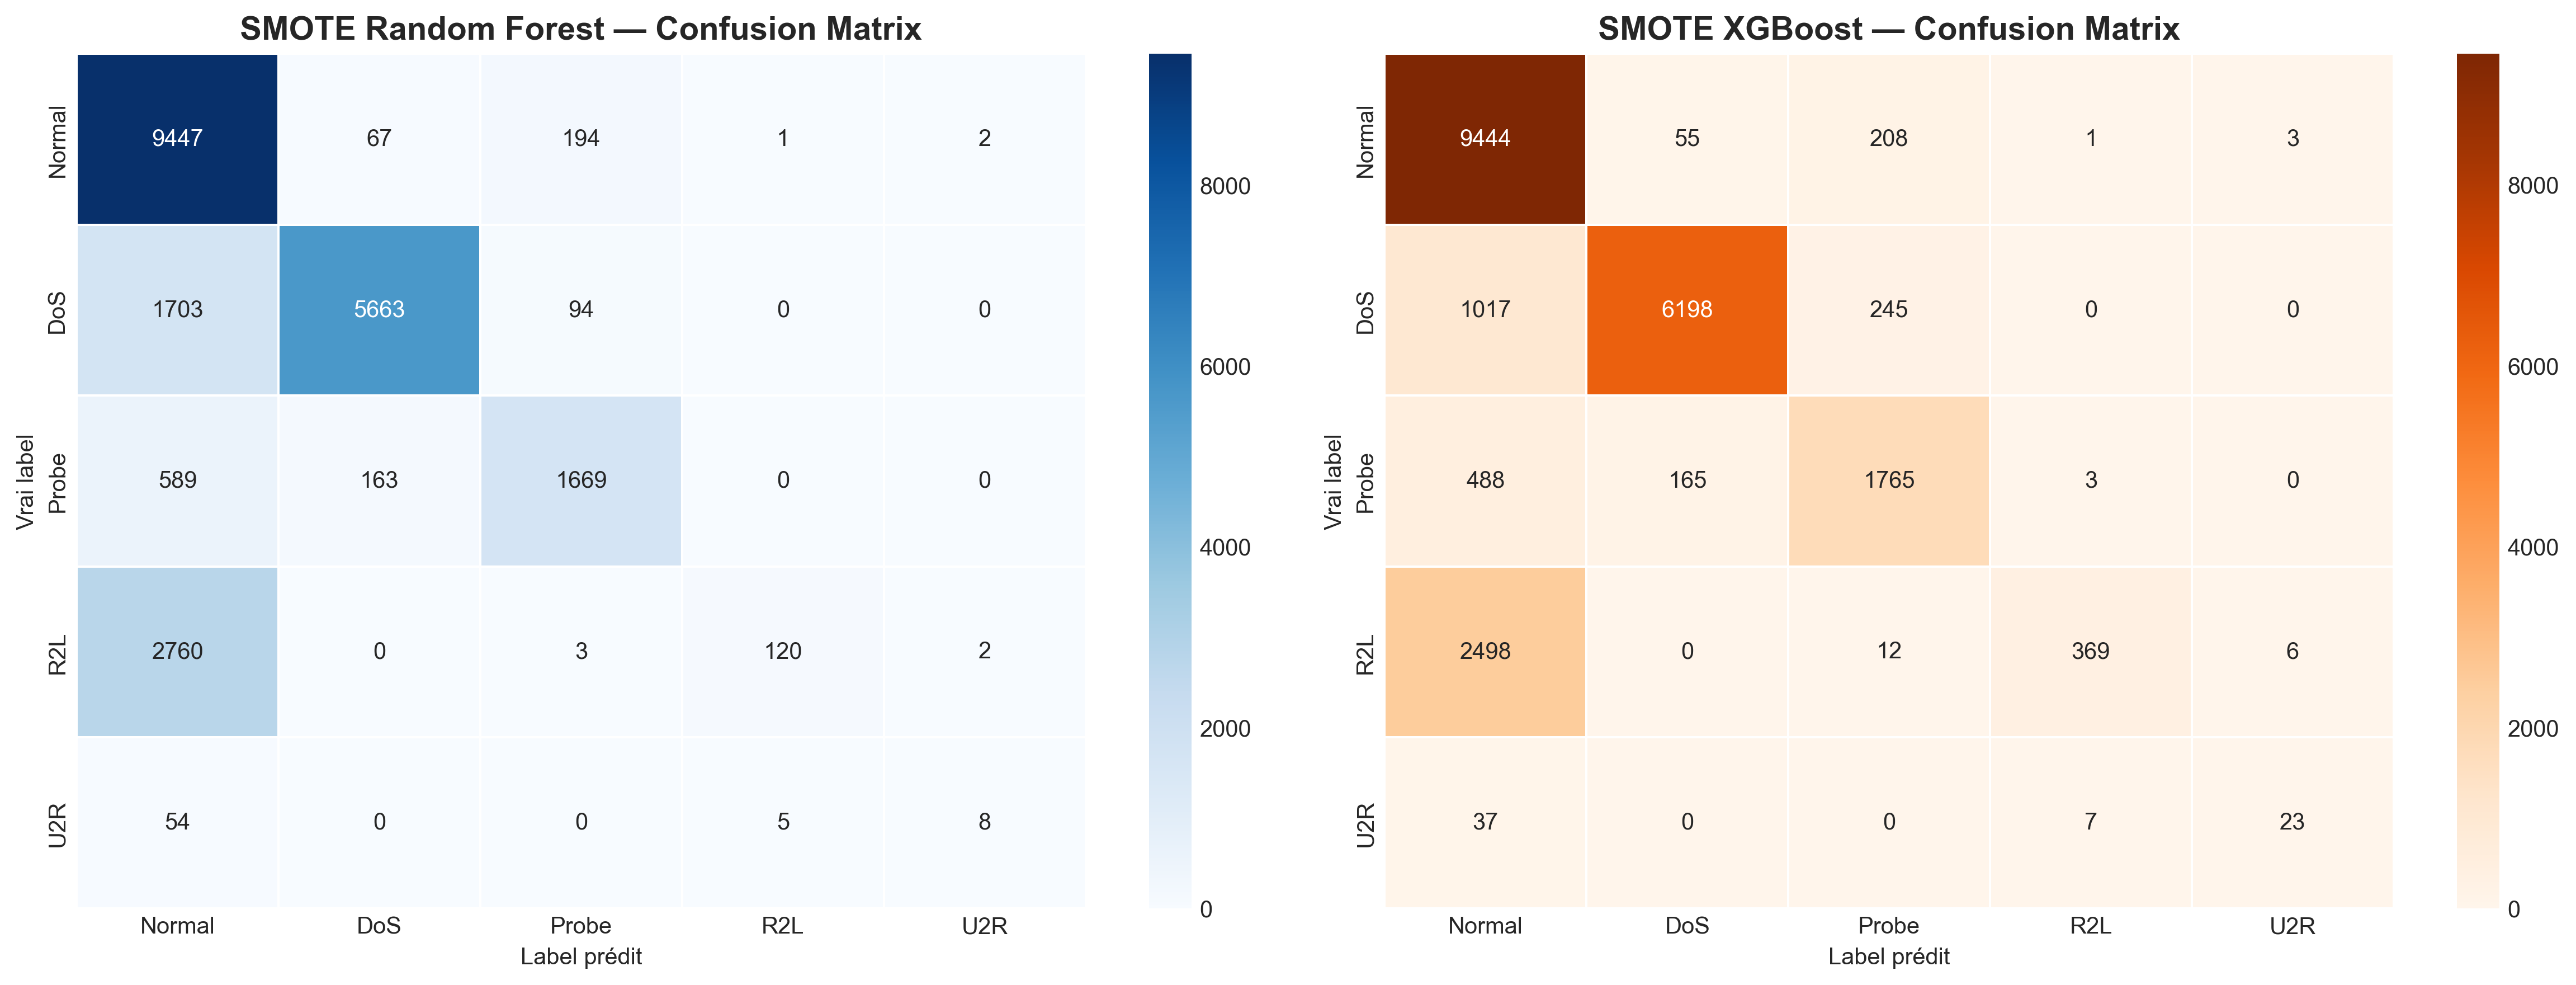
\includegraphics[width=\textwidth]{../reports/confusion_matrices_optimized.png}
    \caption{Matrices de confusion de RF (gauche) et XGBoost (droite).}
    \label{fig:confusion}
\end{figure}

Les attaques R2L (ex: exploitation de failles FTP ou tentatives d'accès par mot de passe) sont majoritairement confondues avec du trafic "Normal". D'un point de vue réseau (sans inspection profonde de la charge utile), ces connexions ressemblent trait pour trait à une connexion légitime, ce qui confirme la difficulté inhérente au dataset.

\section{Importance des caractéristiques}

La Figure~\ref{fig:importance} présente les "Top 20 Features" retenues par XGBoost.

\begin{figure}[H]
    \centering
    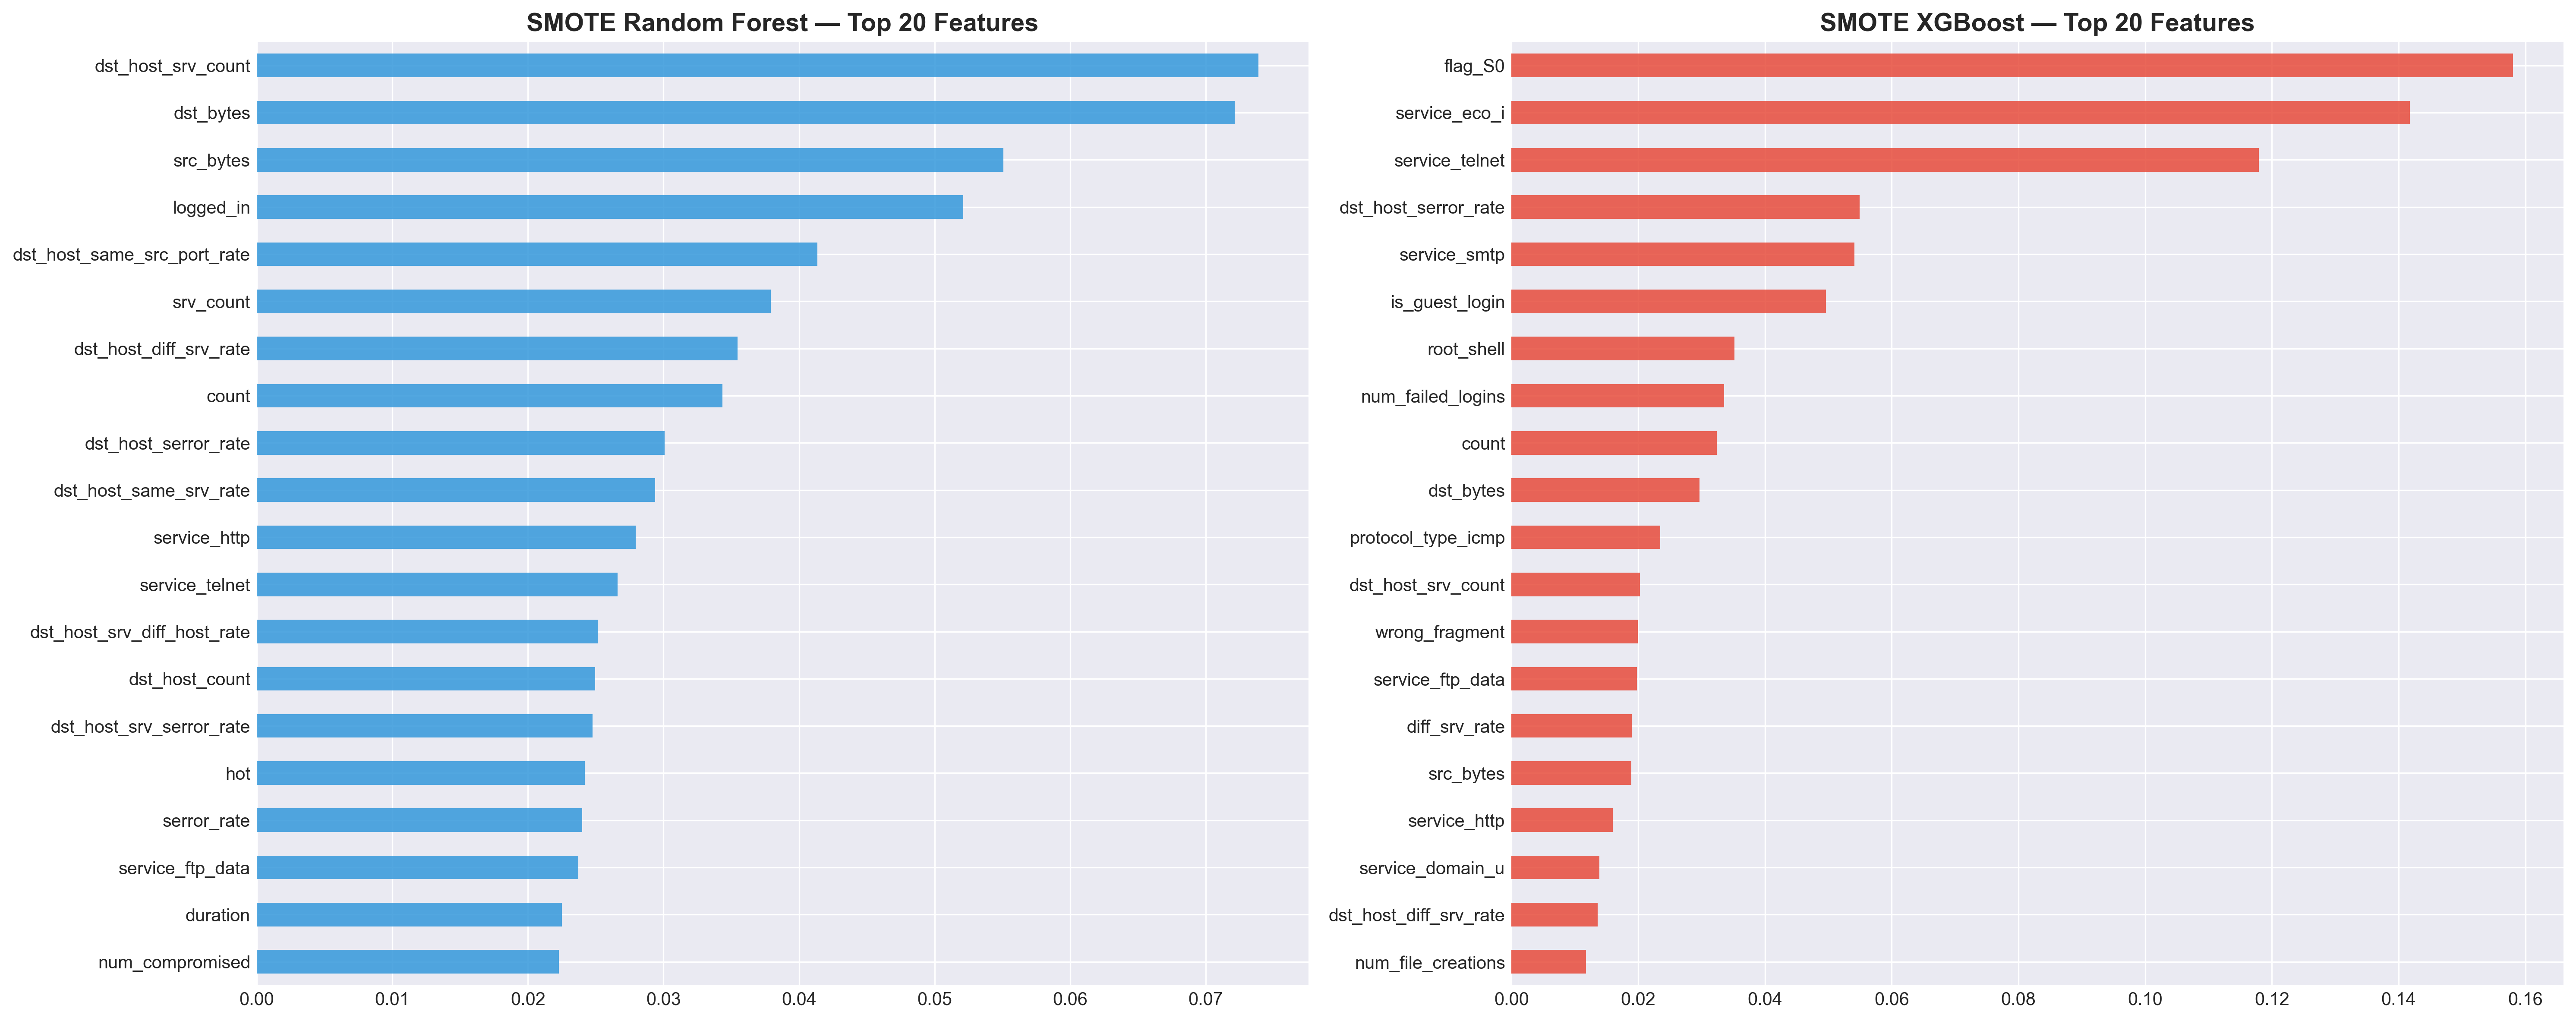
\includegraphics[width=\textwidth]{../reports/feature_importance_optimized.png}
    \caption{Top 20 des caractéristiques les plus importantes (XGBoost à droite).}
    \label{fig:importance}
\end{figure}

Il est intéressant de noter que le modèle s'appuie massivement sur des caractéristiques \textbf{dérivées} (taux d'erreurs SYN, ratio de services) plutôt que sur des ports bruts. C'est ce qui lui confère sa capacité de détection comportementale et sa robustesse face au polymorphisme des attaques.


% ═══════════════════════════════════════════
% CHAPITRE 5 — DÉPLOIEMENT MLOps
% ═══════════════════════════════════════════
\chapter{Industrialisation (MLOps) et Déploiement}

La valeur d'un modèle d'apprentissage réside dans sa capacité à être interrogé en production. Ce chapitre décrit l'architecture d'industrialisation mise en place.

\section{API Asynchrone : FastAPI}

Le modèle entraîné (sérialisé via \texttt{joblib}) est exposé via une API REST développée avec \textbf{FastAPI}. Une attention particulière a été portée à l'optimisation mémoire :
\begin{lstlisting}[caption={Extrait : Gestion de cycle de vie asynchrone}]
@asynccontextmanager
async def lifespan(app: FastAPI):
    global model, scaler, model_columns
    model = joblib.load('models/best_model_cv.pkl')
    scaler = joblib.load('models/scaler.pkl')
    yield
    # Nettoyage à l'arrêt
\end{lstlisting}
Le modèle lourd n'est monté en RAM qu'une seule fois au démarrage du serveur (\textit{Cold Start}), permettant ensuite de traiter les requêtes HTTP d'inférence en quelques millisecondes.

\section{Tableau de bord de type SOC}

Pour visualiser les détections, un tableau de bord a été développé en HTML/JS vanilla. Il interroge l'API à très haute fréquence (simulation d'un flux continu), et propose :
\begin{itemize}
    \item Un suivi des latences en temps réel.
    \item Une jauge dynamique de niveau de menace basée sur le ratio d'attaques récentes.
    \item Un terminal de logs inspiré des interfaces de centres opérationnels de sécurité (SOC).
\end{itemize}

\section{Conteneurisation via Docker}

L'intégralité du pipeline applicatif est orchestrée avec \textbf{Docker}. L'utilisation d'un \texttt{docker-compose.yml} sépare l'environnement en microservices (API Python + Serveur Web Nginx).

Le déploiement sur n'importe quel serveur s'effectue via la commande :
\begin{lstlisting}[language=bash, numbers=none]
cd docker && docker-compose up -d --build
\end{lstlisting}
Cette conteneurisation garantit une reproductibilité stricte, indépendante du système hôte, et supprime le problème classique du "ça marche sur ma machine".


% ═══════════════════════════════════════════
% CHAPITRE 6 — CONCLUSION ET LIMITES
% ═══════════════════════════════════════════
\chapter{Conclusion et Perspectives}

\section{Bilan du projet}

Ce projet a couvert l'ensemble du cycle de vie d'une solution de Machine Learning pour la cybersécurité. Face aux écueils classiques du dataset NSL-KDD, l'utilisation de XGBoost couplée à un pipeline SMOTE intègre a prouvé son efficacité. En passant d'un F1-Score anecdotique à un score de 0,46 sur les attaques ultra-minoritaires (U2R), le modèle a démontré qu'il n'avait pas simplement mémorisé la classe majoritaire, mais qu'il avait extrait une véritable sémantique de l'intrusion. Le déploiement complet via FastAPI et Docker vient asseoir la viabilité opérationnelle de cette approche.

\section{Limites structurelles et axes d'amélioration critiques}

En tant que projet d'ingénierie, il est essentiel de souligner de manière critique les limites actuelles du système :

\begin{enumerate}
    \item \textbf{Le biais temporel (Look-ahead Bias)} : Bien qu'académiquement standard sur NSL-KDD, l'utilisation d'un \texttt{StratifiedKFold} pour la validation croisée d'un trafic réseau implique d'utiliser des données du "futur" pour prédire des données du "passé". En production, une division strictement chronologique (\textit{TimeSeriesSplit}) serait impérative.
    
    \item \textbf{Absence de "Cost-Sensitive Learning"} : En cybersécurité, un Faux Négatif (intrusion non détectée) coûte infiniment plus cher qu'un Faux Positif (alerte injustifiée). Le seuil de décision par défaut de XGBoost (0.5) devrait idéalement être abaissé manuellement pour privilégier le "Recall" (Rappel) des attaques critiques, au détriment de l'Exactitude globale.
    
    \item \textbf{Explicabilité (XAI)} : Pour qu'un opérateur réseau fasse confiance à un modèle, la prédiction doit être explicable. L'intégration d'outils comme \textbf{SHAP} (SHapley Additive exPlanations) pour indiquer \textit{pourquoi} la connexion a été bloquée est aujourd'hui un standard indispensable dans un produit MLOps industriel.
    
    \item \textbf{Latence de prétraitement} : Notre benchmark de performance mesure le temps d'inférence pure du modèle. En production réelle, le temps requis pour parser le paquet brut en temps réel, effectuer le \textit{One-Hot Encoding} et la mise à l'échelle (\textit{Scaling}), ajoutera une surcharge (overhead) non négligeable.
    
    \item \textbf{Surveillance du modèle (Data Drift)} : Les vecteurs d'attaques évoluent quotidiennement. L'architecture actuelle ne prévoit pas de boucle de ré-entraînement automatisée pour pallier la dérive des concepts (\textit{Concept Drift}), ce qui entraînerait une dégradation inévitable de ses performances sur le long terme.
\end{enumerate}

\end{document}
